% Created 2021-03-02 Tue 13:10
% Intended LaTeX compiler: pdflatex
\documentclass[english]{article}
\usepackage[T1, T2A]{fontenc}
\usepackage[lutf8]{luainputenc}
\usepackage[english, russian]{babel}
\usepackage{minted}
\usepackage{graphicx}
\usepackage{longtable}
\usepackage{hyperref}
\usepackage{xcolor}
\usepackage{natbib}
\usepackage{amssymb}
\usepackage{amsmath}
\usepackage{caption}
\usepackage{mathtools}
\usepackage{amsthm}
\usepackage{tikz}
\usepackage{grffile}
\usepackage{extarrows}
\usepackage{wrapfig}
\usepackage{rotating}
\usepackage{placeins}
\usepackage[normalem]{ulem}
\usepackage{amsmath}
\usepackage{textcomp}
\usepackage{capt-of}

\usepackage{geometry}
\geometry{a4paper,left=2.5cm,top=2cm,right=2.5cm,bottom=2cm,marginparsep=7pt, marginparwidth=.6in}

 \usepackage{hyperref}
 \hypersetup{
     colorlinks=true,
     linkcolor=blue,
     filecolor=orange,
     citecolor=black,      
     urlcolor=cyan,
     }

\usetikzlibrary{decorations.markings}
\usetikzlibrary{cd}
\usetikzlibrary{patterns}

\newcommand\addtag{\refstepcounter{equation}\tag{\theequation}}
\newcommand{\eqrefoffset}[1]{\addtocounter{equation}{-#1}(\arabic{equation}\addtocounter{equation}{#1})}


\newcommand{\R}{\mathbb{R}}
\renewcommand{\C}{\mathbb{C}}
\newcommand{\N}{\mathbb{N}}
\newcommand{\rank}{\text{rank}}
\newcommand{\const}{\text{const}}
\newcommand{\grad}{\text{grad}}

\theoremstyle{plain}
\newtheorem{axiom}{Аксиома}
\newtheorem{lemma}{Лемма}
\newtheorem{manuallemmainner}{Лемма}
\newenvironment{manuallemma}[1]{%
  \renewcommand\themanuallemmainner{#1}%
  \manuallemmainner
}{\endmanuallemmainner}

\theoremstyle{remark}
\newtheorem*{remark}{Примечание}
\newtheorem*{solution}{Решение}
\newtheorem{corollary}{Следствие}[theorem]
\newtheorem*{examp}{Пример}
\newtheorem*{observation}{Наблюдение}

\theoremstyle{definition}
\newtheorem{task}{Задача}
\newtheorem{theorem}{Теорема}[section]
\newtheorem*{definition}{Определение}
\newtheorem*{symb}{Обозначение}
\newtheorem{manualtheoreminner}{Теорема}
\newenvironment{manualtheorem}[1]{%
  \renewcommand\themanualtheoreminner{#1}%
  \manualtheoreminner
}{\endmanualtheoreminner}
\captionsetup{justification=centering,margin=2cm}
\newenvironment{colored}[1]{\color{#1}}{}

\tikzset{->-/.style={decoration={
  markings,
  mark=at position .5 with {\arrow{>}}},postaction={decorate}}}
\makeatletter
\newcommand*{\relrelbarsep}{.386ex}
\newcommand*{\relrelbar}{%
  \mathrel{%
    \mathpalette\@relrelbar\relrelbarsep
  }%
}
\newcommand*{\@relrelbar}[2]{%
  \raise#2\hbox to 0pt{$\m@th#1\relbar$\hss}%
  \lower#2\hbox{$\m@th#1\relbar$}%
}
\providecommand*{\rightrightarrowsfill@}{%
  \arrowfill@\relrelbar\relrelbar\rightrightarrows
}
\providecommand*{\leftleftarrowsfill@}{%
  \arrowfill@\leftleftarrows\relrelbar\relrelbar
}
\providecommand*{\xrightrightarrows}[2][]{%
  \ext@arrow 0359\rightrightarrowsfill@{#1}{#2}%
}
\providecommand*{\xleftleftarrows}[2][]{%
  \ext@arrow 3095\leftleftarrowsfill@{#1}{#2}%
}
\makeatother
\author{Ilya Yaroshevskiy}
\date{\today}
\title{Практика 4}
\hypersetup{
 pdfauthor={Ilya Yaroshevskiy},
 pdftitle={Практика 4},
 pdfkeywords={},
 pdfsubject={},
 pdfcreator={Emacs 28.0.50 (Org mode )}, 
 pdflang={English}}
\begin{document}

\maketitle
\tableofcontents

\begin{task}
Первый цех производит 50\% деталей, второй цех - 30\%, трейтий цех -
20\%. Брак в первом цехе - 3\%, во втором - 5\%, в тертьем - 4\%. Найти
вероятность что деталь без брака.
\end{task}
\begin{solution}
\(A\) --- деталь с браком \\
\(B_i\) --- произвдена в \(i\text{-том}\) цехе
\[ P(B_1) = 0.5 \]
\[ P(B_2) = 0.3 \]
\[ P(B_3) = 0.2 \]
\[ P(A|B_1) = 0.03 \]
\[ P(A|B_2) = 0.05 \]
\[ P(A|B_3) = 0.04 \]
\[ P(A) = P(B_1)P(A|B_1) + P(B_2)P(A|B_2) + P(B_3)P(A|B_3) = 0.5\cdot0.03 + 0.3\cdot0.05 + 0.2\cdot0.04 = 0.038 \]
\[ P(\overline{A}) = 1 - P(A) = 0.962 \]
\end{solution}

\begin{task}
В группе 2 отличника, 5 хорошистов и 3 троешника. Вероятности решить
задачу соответственно 0.9, 0.7, 0.4. Наугад вызванный студент
решил. Ворятность что это отличник
\end{task}
\begin{solution}
\(A\) --- решил задачу, \(H_i\) --- чувак
\[ P(A|H_1) = 0.9 \]
\[ P(A|H_2) = 0.7 \]
\[ P(A|H_3) = 0.4 \]
\[ P(H_1) = 0.2 \]
\[ P(H_2) = 0.5 \]
\[ P(H_3) = 0.3 \]
\[ P(A) = P(A|H_1)P(H_1) + P(A|H_2)P(H_2) + P(A|H_3)P(H_3) = 0.9\cdot0.2 + 0.7\cdot0.5 + 0.4\cdot0.3 = 0.65\]
\[ P(H_1|A) = \frac{P(A|H_1)P(H_1)}{P(A)} = \frac{0.9\cdot0.2}{0.65} = \frac{18}{65} \]
\end{solution}
\begin{task}
Веротяность попадания стрелка в цель --- 0.5. Стрелок подбрасывает две
монеты, делает число выстрелов равное удвоенному числу гербов. Найти
веротяность что стрелок попал в цель.
\end{task}
\begin{solution}
\(A\) --- попал хотябы раз, \(H_i\) --- вероятность числа гребов соотвественно \(0, 2, 2, 4\)
\[ P(H_i) = 0.25 \]
\[ P(A|H_1) = 0 \]
Считаем через обратную, т.е. через веротяность что не попал ни разу.
\[ P(A|H_2) = 0.5\cdot2 - 0.5^2 \]
\[ P(A|H_3) = 0.5\cdot2 - 0.5^2 \]
\[ P(A|H_4) = 0.5\cdot4 - 0.5^4 \]
\[ P(A) = P(A|H_1)P(H_1) + P(A|H_2)P(H_2) + P(A|H_3)P(H_3) + P(A|H_4)P(H_4) \]
\end{solution}
\begin{task}
В первой коробке 4 белых и 1 черный шар, во второй --- 3 белых, 2
черных, в третьей -- 1 белый, 4 черных. Из наугда выбранной коробки
взяли два шара, они оказались белыми. Найти вероятность того что была выбрана вторая коробка.
\end{task}
\begin{solution}
\(A\) --- было выбрано 2 белых шара, \(H_i\) --- \(i\text{-тая}\) коробка
\[ P(H_1) = \frac{1}{3} \]
\[ P(H_2) = \frac{1}{3} \]
\[ P(H_3) = \frac{1}{3} \]
\[ P(A|H_1) = \frac{4}{5}\cdot\frac{3}{4} \]
\[ P(A|H_2) = \frac{3}{5}\cdot\frac{2}{4} \]
\[ P(A|H_3) = P(H_1)P(A|H_1) + P(H_2)P(A|H_2) + P(H_3)P(A|H_3) = \frac{2}{10} + \frac{1}{10} + 0 = \frac{3}{10} \]
\[ P(A) = \frac{P(A|H_2)P(H_2)}{P(A)} = \frac{\frac{1}{10}}{\frac{3}{10}} = \frac{1}{3} \]
\end{solution}
\begin{task}
На шахматную доску наугад поставили короля и коня. Найти вероятность того, что конь объявит шах.
\end{task}
\begin{solution}
Разбиваем на зоны начиная с краев.
\begin{center}
\begin{tabular}{r|rr|}
Зона & Число клеток в зоне & Число бьющихся клеток\\
\hline
1 & 4 & 2\\
2 & 8 & 3\\
3 & 20 & 4\\
4 & 16 & 6\\
5 & 16 & 8\\
\end{tabular}
\end{center}
\[ P(A) = \frac{4}{64}\cdot\frac{2}{63} + \frac{8}{64}\cdot\frac{3}{63} + \frac{20}{64}\cdot\frac{4}{63} + \frac{16}{64}\cdot\frac{6}{63} + \frac{16}{64}\cdot\frac{8}{63} = \frac{1}{12} \]
\end{solution}
\begin{task}
\-
\begin{center}
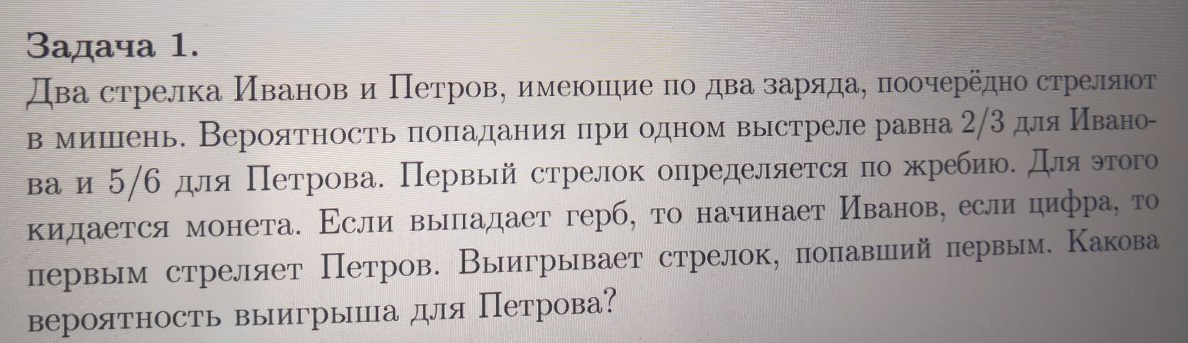
\includegraphics[width=.9\linewidth]{4_1.png}
\end{center}
Петров выиграл. Какова вероятность что он стрелял первым
\end{task}
\begin{solution}
\(Pe\) --- Петров попал, \(Iv\) --- иванов попал, \(H_1\) --- Петров стрелял
первый, \(H_2\) --- Иванов стрелял первый, \(A\) --- Выиграл Петров
\[ P(H_1) = \frac{1}{2} \]
\[ P(H_2) = \frac{1}{2} \]
\[ P(A|H_1) = P(Pe + \overline{Pe}\cdot\overline{Iv}\cdot Pe) = P(Pe) + P(\overline{Pe}\cdot\overline{Iv}\cdot Pe) = \frac{95}{36\cdot 3} \]
\[ P(A|H_2) = P(\overline{Iv}\cdot Pe + \overline{Iv}\cdot\overline{Pe}\cdot\overline{Iv}\cdot Pe) = \frac{95}{18^2}\]
\[ P(H_1|A) = \frac{3}{4} \]
\end{solution}
\begin{task}
В студии три двери, за одной приз. Игрок указывает дверь, ведущий
открвается одну из оставшихся и показывает что там приза нет. После
чего предлагает игроку поменять свой выбор. Стоит ли это делать?
\end{task}
\begin{solution}
\begin{enumerate}
\item \(H_1\) --- игрок угадал, \(H_2\) --- игрок не угадал, \(A\) --- ведущий открыл двеоь без приза
\[ P(H_1) = \frac{1}{3} \]
\[ P(H_2) = \frac{2}{3} \]
\[ P(A|H_1) = 1 \]
\[ P(A|H_2) = \frac{1}{2}\color{red}??? \]
\[ P(H_1|A) = \frac{P(A|H_1)P(H_1)}{P(A|H_1)P(H_1) + P(A|H_2)P(H_2)} = \frac{1}{2} \]
\color{red} \(A\) --- не случайное событие \(\Rightarrow\) нельзя применять формулу Баеса \color{black}
\item Статистически \\
\(300\) экспериментов, \(100\) угадал, \(100\) не угадал, \(\frac{200}{300} = \frac{2}{3}\)
\end{enumerate}
\end{solution}
\end{document}
